\documentclass[aspectratio=169]{beamer}

% ---------- ENCODING & FONTS ----------
\usepackage[utf8]{inputenc}
\usepackage[T1]{fontenc}

% ---------- THEME & LOOK ----------
\usetheme{Madrid}
\usecolortheme{seahorse}
\usefonttheme{professionalfonts}
\setbeamertemplate{navigation symbols}{}
\setbeamercovered{transparent}
\setbeamertemplate{itemize items}[circle]
\setbeamertemplate{enumerate items}[default]
\setlength{\parskip}{0.25em}

% ---------- COLORS ----------
\definecolor{accent}{RGB}{0,92,184}
\definecolor{soft}{RGB}{233,244,255}
\definecolor{canadared}{RGB}{196,30,58}
\definecolor{leafgreen}{RGB}{0,130,80}
\definecolor{goldenrod}{RGB}{218,165,32}
\definecolor{deeporange}{RGB}{220,90,20}
\definecolor{shiftpurple}{RGB}{130,50,180}
\definecolor{tealblue}{RGB}{0,128,128}
\definecolor{lightred}{RGB}{245,210,210}
\setbeamercolor{structure}{fg=accent}
\setbeamercolor{title}{fg=white,bg=accent}
\setbeamercolor{frametitle}{fg=accent}
\setbeamercolor{block title}{bg=accent!12,fg=accent}
\setbeamercolor{block body}{bg=soft}

% ---------- PACKAGES ----------
\usepackage{booktabs}
\usepackage{amsmath, amssymb}
\usepackage{array}
\usepackage{multirow}
\usepackage{hyperref}
\usepackage{tikz}
\usepackage{pgfplots}
\pgfplotsset{compat=1.18}
\usetikzlibrary{arrows.meta, positioning, calc, shapes.geometric}
\hypersetup{colorlinks=true,linkcolor=accent,urlcolor=accent}

% ---------- SAFE TRANSITION FALLBACK ----------
\makeatletter
\@ifundefined{transfade}{\newcommand{\transfade}[1][]{}}{}
\makeatother

% ---------- TITLE ----------
\title{\textbf{Aggregate Demand and Aggregate Supply Analysis}}
\subtitle{{\large ECON 101 -- Principles of Macroeconomics}}
\author{Muhebullah Karimzada}
\date{Spring 2026}

% ============================================================
\begin{document}
% ============================================================

\begin{frame}[plain]
  \titlepage
\end{frame}

\begin{frame}{Chapter Outline}
\transfade
\begin{itemize}
  \item \textbf{9.1} Aggregate Demand
  \item \textbf{9.2} Aggregate Supply
  \item \textbf{9.3} Macroeconomic Equilibrium in the Long Run and the Short Run
\end{itemize}
\end{frame}

% ============================================================
\section{9.1 Aggregate Demand}
% ============================================================

\begin{frame}{9.1 Learning Objective}
\transfade
\begin{block}{Goal}
Identify the determinants of aggregate demand and distinguish between a movement along the AD curve and a shift.
\end{block}
\begin{itemize}
  \item Chapter 8 derived the AD curve from the AE model.
  \item This chapter:
  \begin{itemize}
    \item Analyzes what \textbf{shifts} the AD curve,
    \item Introduces the \textbf{aggregate supply curves} (SRAS and LRAS),
    \item Combines AD and AS to find \textbf{macroeconomic equilibrium}.
  \end{itemize}
\end{itemize}
\end{frame}

\begin{frame}{Figure 9.1 -- The Aggregate Demand Curve}
\begin{center}
\begin{tikzpicture}
\begin{axis}[
  width=0.72\textwidth, height=0.72\textheight,
  xlabel={Real GDP (\$billions)},
  ylabel={Price Level ($P$, CPI Index)},
  xmin=0, xmax=3000, ymin=90, ymax=180,
  xtick={500,1000,1500,2000,2500},
  ytick={100,110,120,130,140,150,160,170},
  grid=major, grid style={dotted,gray!40},
  tick label style={font=\small},
  label style={font=\small},
  title style={font=\small\bfseries},
  title={The Aggregate Demand Curve Slopes Downward}
]
\addplot[deeporange, very thick, smooth, domain=300:2800, samples=50]
  {280 - 0.06*x}
  node[right, font=\small, color=deeporange] {\textbf{AD}};
\node[font=\small, fill=soft, draw=deeporange, rounded corners, align=left]
  at (axis cs:2200,160) {Higher $P$ reduces:\\
  $\bullet$ Wealth $\Rightarrow \downarrow C$\\
  $\bullet$ Interest rate $\Rightarrow \downarrow I$\\
  $\bullet$ Intl.\ trade $\Rightarrow \downarrow NX$};
\end{axis}
\end{tikzpicture}
\end{center}
\end{frame}

\begin{frame}{Why the AD Curve Slopes Downward: Three Effects}
\transfade
\begin{enumerate}
  \item \textbf{Wealth Effect} $\Rightarrow$ lower $C$
  \begin{itemize}
    \item Higher $P$ erodes the real value of nominal assets (cash, savings accounts).
    \item Canadians feel poorer $\Rightarrow$ spend less.
    \item \textbf{Example:} if CPI rises by 10\%, \$50{,}000 in a savings account buys 10\% less.
  \end{itemize}
  \item \textbf{Interest-Rate Effect} $\Rightarrow$ lower $I$
  \begin{itemize}
    \item Higher $P$ raises money demand $\Rightarrow$ interest rates rise $\Rightarrow$ investment falls.
    \item \textbf{Canada 2022}: as inflation rose, interest rates followed --- new mortgages and business loans became expensive, crushing investment.
  \end{itemize}
  \item \textbf{International-Trade Effect} $\Rightarrow$ lower $NX$
  \begin{itemize}
    \item Canadian goods more expensive relative to U.S./world goods.
    \item Exports fall; imports rise $\Rightarrow$ NX falls.
    \item \textbf{Example:} CAD lumber becomes expensive for American homebuilders.
  \end{itemize}
\end{enumerate}
\end{frame}

\begin{frame}{Variables That Shift the AD Curve (1/2)}
\transfade
\begin{center}
\begin{tabular}{p{0.42\linewidth} p{0.12\linewidth} p{0.38\linewidth}}
\toprule
\textbf{Change} & \textbf{AD shifts} & \textbf{Canadian example} \\
\midrule
BoC \textbf{cuts} overnight rate & Right $\to$ & 2020: cut to 0.25\% to boost AD \\
BoC \textbf{raises} overnight rate & Left $\leftarrow$ & 2022--23: hikes to 5\% to cool inflation \\
Federal gov't \textbf{increases} spending & Right $\to$ & 2020: \$314B COVID stimulus \\
Federal gov't \textbf{cuts} spending & Left $\leftarrow$ & 1990s austerity under Martin \\
Personal income tax \textbf{cut} & Right $\to$ & GST cut from 7\% to 5\% (2006--08) \\
Personal income tax \textbf{increase} & Left $\leftarrow$ & Higher OAS clawback \\
Households expect \textbf{higher} income & Right $\to$ & 2021 pent-up demand reopening \\
U.S. economy \textbf{slows} sharply & Left $\leftarrow$ & 2008--09 U.S. recession hurt Canada \\
CAD \textbf{depreciates} & Right $\to$ & Cheaper exports boost AD \\
\bottomrule
\end{tabular}
\end{center}
\end{frame}

\begin{frame}{Variables That Shift the AD Curve (2/2)}
\transfade
\begin{center}
\begin{tikzpicture}
\begin{axis}[
  width=0.80\textwidth, height=0.70\textheight,
  xlabel={Real GDP},
  ylabel={Price Level},
  xmin=0, xmax=10, ymin=0, ymax=10,
  xtick=\empty, ytick=\empty,
  axis lines=left,
  label style={font=\small},
  title style={font=\small\bfseries},
  title={Shifts of the Aggregate Demand Curve}
]
% Original AD
\addplot[accent, very thick, domain=0:9] {9 - x}
  node[right, font=\small, color=accent] {$AD$};
% Right shift
\addplot[leafgreen, very thick, dashed, domain=0:9] {11 - x}
  node[right, font=\small, color=leafgreen] {$AD'$ (expansionary)};
% Left shift
\addplot[canadared, very thick, dashed, domain=0:9] {7 - x}
  node[right, font=\small, color=canadared] {$AD''$ (contractionary)};
% Arrows
\draw[->, very thick, leafgreen] (axis cs:3,7) -- (axis cs:5,7)
  node[above, midway, font=\tiny, color=leafgreen] {\footnotesize $\to$};
\draw[->, very thick, canadared] (axis cs:3,5) -- (axis cs:1,5)
  node[above, midway, font=\tiny, color=canadared] {\footnotesize $\leftarrow$};
\node[font=\tiny, fill=leafgreen!10, draw=leafgreen, rounded corners, align=center]
  at (axis cs:7,9) {Expansionary:\\$\uparrow G$, $\downarrow i$, $\downarrow T$};
\node[font=\tiny, fill=lightred, draw=canadared, rounded corners, align=center]
  at (axis cs:1.5,3) {Contractionary:\\$\downarrow G$, $\uparrow i$, $\uparrow T$};
\end{axis}
\end{tikzpicture}
\end{center}
\end{frame}

% ============================================================
\section{9.2 Aggregate Supply}
% ============================================================

\begin{frame}{9.2 Learning Objective}
\transfade
\begin{block}{Goal}
Identify the determinants of aggregate supply and distinguish between SRAS and LRAS.
\end{block}
\begin{itemize}
  \item \textbf{Long-run aggregate supply (LRAS):}
  \begin{itemize}
    \item Vertical line at \textbf{potential GDP} --- determined by labour, capital, and technology.
    \item \alert{Not affected} by the price level in the long run.
  \end{itemize}
  \item \textbf{Short-run aggregate supply (SRAS):}
  \begin{itemize}
    \item Upward-sloping --- as prices of final goods rise, input prices (especially wages) are slow to adjust, so profits rise and firms produce more.
  \end{itemize}
\end{itemize}
\end{frame}

\begin{frame}{Figure 9.2 -- LRAS and SRAS Curves}
\begin{center}
\begin{tikzpicture}
\begin{axis}[
  width=0.78\textwidth, height=0.72\textheight,
  xlabel={Real GDP (\$billions)},
  ylabel={Price Level ($P$)},
  xmin=0, xmax=3000, ymin=80, ymax=200,
  xtick={500,1000,1500,2000,2500},
  ytick={90,110,130,150,170,190},
  grid=major, grid style={dotted,gray!40},
  tick label style={font=\small},
  label style={font=\small},
  title style={font=\small\bfseries},
  title={Long-Run Supply is Vertical; Short-Run Supply Slopes Up}
]
% LRAS (vertical at potential GDP = 2000)
\addplot[shiftpurple, very thick] coordinates {(2000,80)(2000,200)};
\node[right, font=\small, color=shiftpurple, align=left] at (axis cs:2050,170) {\textbf{LRAS}\\(Potential\\GDP)};
% SRAS (upward sloping)
\addplot[goldenrod, very thick, domain=500:2800, samples=40] {0.05*x + 30}
  node[right, font=\small, color=goldenrod] {\textbf{SRAS}};
\node[font=\small, fill=soft, draw=shiftpurple, rounded corners, align=center]
  at (axis cs:900,175) {At potential GDP:\\full employment,\\normal capacity};
\end{axis}
\end{tikzpicture}
\end{center}
\end{frame}

\begin{frame}{Why Is SRAS Upward Sloping?}
\transfade
\begin{itemize}
  \item When the price level rises, firms are willing to produce more \textbf{in the short run}. Why?
\end{itemize}
\begin{enumerate}
  \item \textbf{Sticky wages (contracts):}
  \begin{itemize}
    \item Most Canadian workers have annual salary reviews or multi-year collective agreements.
    \item When $P$ rises unexpectedly, wages stay fixed in the short run $\Rightarrow$ real wages fall $\Rightarrow$ labour is cheaper $\Rightarrow$ firms hire more and produce more.
  \end{itemize}
  \item \textbf{Slow wage adjustment:}
  \begin{itemize}
    \item Firms rarely cut nominal wages (damages morale). Adjustment is gradual.
  \end{itemize}
  \item \textbf{Menu costs:}
  \begin{itemize}
    \item Changing prices is costly (reprinting catalogues, updating point-of-sale systems).
    \item For small demand increases, firms adjust quantity rather than price.
  \end{itemize}
\end{enumerate}
\end{frame}

\begin{frame}{Variables That Shift SRAS}
\transfade
\begin{center}
\small
\begin{tabular}{p{0.40\linewidth} p{0.10\linewidth} p{0.42\linewidth}}
\toprule
\textbf{Change} & \textbf{Shift} & \textbf{Example} \\
\midrule
Larger labour force or capital stock & Right & Immigration surge (Canada 2022--24: +1.2M/yr) \\
Better technology & Right & AI-assisted software development \\
Decrease in oil/energy prices & Right & OPEC supply increase \\
Increase in oil/energy prices & Left & Russia--Ukraine war 2022 \\
Workers expect higher $P$ (wage push) & Left & Union wage demands after 8.1\% inflation \\
COVID shutdowns & Left & Factories closed, supply chains disrupted \\
Decrease in labour force & Left & Baby boomer retirements \\
\bottomrule
\end{tabular}
\end{center}
\vspace{0.3em}
\begin{itemize}
  \item \textbf{Key rule:} anything that raises production \textit{costs} (holding output prices constant) shifts SRAS \textbf{left}; anything that lowers costs shifts SRAS \textbf{right}.
\end{itemize}
\end{frame}

% ============================================================
\section{9.3 Macroeconomic Equilibrium}
% ============================================================

\begin{frame}{9.3 Learning Objective}
\transfade
\begin{block}{Goal}
Use the AD--AS model to illustrate short-run and long-run macroeconomic equilibrium.
\end{block}
\begin{itemize}
  \item \textbf{Short-run equilibrium}: AD intersects SRAS.
  \begin{itemize}
    \item Real GDP may be above or below potential GDP.
  \end{itemize}
  \item \textbf{Long-run equilibrium}: AD, SRAS, and LRAS all intersect.
  \begin{itemize}
    \item Real GDP $=$ potential GDP; wages and prices fully adjusted.
  \end{itemize}
\end{itemize}
\end{frame}

\begin{frame}{Figure 9.3 -- Long-Run Macroeconomic Equilibrium}
\begin{center}
\begin{tikzpicture}
\begin{axis}[
  width=0.78\textwidth, height=0.72\textheight,
  xlabel={Real GDP (\$billions)},
  ylabel={Price Level ($P$)},
  xmin=0, xmax=3000, ymin=80, ymax=200,
  xtick={500,1000,1500,2000,2500},
  ytick={90,110,130,150,170,190},
  grid=major, grid style={dotted,gray!40},
  tick label style={font=\small},
  label style={font=\small},
  title style={font=\small\bfseries},
  title={Long-Run Equilibrium: AD $\cap$ SRAS $\cap$ LRAS}
]
\addplot[shiftpurple, very thick] coordinates {(2000,80)(2000,200)};
\node[right, font=\tiny, color=shiftpurple] at (axis cs:2050,180) {LRAS};
\addplot[goldenrod, very thick, domain=500:2800] {0.05*x + 30}
  node[right, font=\tiny, color=goldenrod] {SRAS};
% AD: P=240-0.055*x; at x=2000: P=240-110=130. SRAS at x=2000: P=0.05*2000+30=130. Consistent.
\addplot[deeporange, very thick, domain=500:2800] {240 - 0.055*x}
  node[right, font=\tiny, color=deeporange] {\textbf{AD}};
\addplot[accent, only marks, mark=*, mark size=4pt] coordinates {(2000,130)};
\draw[dashed, accent] (axis cs:2000,130) -- (axis cs:0,130)
  node[left, font=\small, color=accent] {$P^*=130$};
\draw[dashed, accent] (axis cs:2000,130) -- (axis cs:2000,80)
  node[below, font=\tiny, color=accent] {$Y^*=\$2000B$};
\node[font=\small, fill=soft, draw=accent, rounded corners, align=center]
  at (axis cs:700,180) {\textbf{Long-Run Eq.}\\AD $\cap$ SRAS $\cap$ LRAS\\$Y^* = \$2000B,\ P^* = 130$};
\end{axis}
\end{tikzpicture}
\end{center}
\end{frame}

\begin{frame}{Figure 9.4 -- Decrease in AD: Canada 2022 Rate Hike Example}
\begin{center}
\begin{tikzpicture}
\begin{axis}[
  width=0.80\textwidth, height=0.70\textheight,
  xlabel={Real GDP (\$billions)},
  ylabel={Price Level ($P$)},
  xmin=0, xmax=3000, ymin=80, ymax=200,
  xtick={500,1000,1500,2000,2500},
  ytick={90,110,130,150,170,190},
  grid=major, grid style={dotted,gray!40},
  tick label style={font=\small},
  label style={font=\small},
  title style={font=\small\bfseries},
  title={BoC Rate Hikes (2022--23) Shifted AD Left, Reducing GDP and Inflation}
]
\addplot[shiftpurple, very thick] coordinates {(2000,80)(2000,200)};
\node[right, font=\tiny, color=shiftpurple] at (axis cs:2050,185) {LRAS};
\addplot[goldenrod, very thick, domain=500:2800] {0.05*x + 30};
\node[right, font=\tiny, color=goldenrod] at (axis cs:2650,163) {SRAS};
% Original AD (slightly right of LRAS - inflationary)
\addplot[accent, very thick, domain=500:2800] {255 - 0.055*x}
  node[right, font=\tiny, color=accent] {$AD_1$ (pre-hike)};
% New AD (shifted left)
\addplot[canadared, very thick, dashed, domain=200:2800] {225 - 0.055*x}
  node[right, font=\tiny, color=canadared] {$AD_2$ (post-hike)};
% Equilibria
% AD1 cap SRAS: 255-0.055x=0.05x+30 => 225=0.105x => x=2143; P=0.05*2143+30=137
\addplot[accent, only marks, mark=*, mark size=3.5pt] coordinates {(2143,137)};
% AD2 cap SRAS: 225-0.055x=0.05x+30 => 195=0.105x => x=1857; P=0.05*1857+30=123
\addplot[canadared, only marks, mark=*, mark size=3.5pt] coordinates {(1857,123)};
\draw[dashed, accent] (axis cs:2143,137)--(axis cs:2143,0) node[below,font=\tiny,color=accent]{$Y_1$};
\draw[dashed, canadared] (axis cs:1857,123)--(axis cs:1857,0) node[below,font=\tiny,color=canadared]{$Y_2$};
\draw[dashed, accent] (axis cs:2143,137)--(axis cs:0,137) node[left,font=\tiny,color=accent]{$P_1$};
\draw[dashed, canadared] (axis cs:1857,123)--(axis cs:0,123) node[left,font=\tiny,color=canadared]{$P_2$};
\draw[->, very thick, canadared] (axis cs:1500,155) -- (axis cs:1200,155)
  node[above, midway, font=\tiny, color=canadared] {AD shifts left};
\node[font=\tiny, fill=lightred, draw=canadared, rounded corners, align=center]
  at (axis cs:700,165) {BoC: 0.25\%$\to$5.0\%\\reduced AD,\\lowered inflation};
\end{axis}
\end{tikzpicture}
\end{center}
\end{frame}

\begin{frame}{Long-Run Adjustment After a Decrease in AD}
\transfade
\begin{itemize}
  \item Short-run: AD shifts left $\Rightarrow$ GDP falls below potential, unemployment rises, $P$ falls.
  \item \textbf{Long-run adjustment:}
  \begin{itemize}
    \item High unemployment $\Rightarrow$ workers accept lower wages.
    \item Lower wages $\Rightarrow$ production costs fall $\Rightarrow$ SRAS shifts \textbf{right}.
    \item SRAS keeps shifting right until $Y = Y^*$ (potential GDP).
    \item Long-run result: \textbf{lower price level}, same real GDP as before.
  \end{itemize}
  \item \textbf{Canadian example (2023--2024):} BoC's rate hikes reduced demand, slowing inflation from 8.1\% (June 2022) to \alert{1.8\%} (Sept 2024) --- but at the cost of unemployment rising from 5.3\% to 6.3\%.
  \begin{itemize}
    \item \textcolor{goldenrod}{Source: Statistics Canada; Bank of Canada MPR (2024).}
  \end{itemize}
\end{itemize}
\end{frame}

\begin{frame}{Figure 9.5 -- Increase in AD: Post-COVID Boom (2021)}
\begin{center}
\begin{tikzpicture}
\begin{axis}[
  width=0.80\textwidth, height=0.70\textheight,
  xlabel={Real GDP (\$billions)},
  ylabel={Price Level ($P$)},
  xmin=0, xmax=3000, ymin=80, ymax=200,
  xtick={500,1000,1500,2000,2500},
  ytick={90,110,130,150,170,190},
  grid=major, grid style={dotted,gray!40},
  tick label style={font=\small},
  label style={font=\small},
  title style={font=\small\bfseries},
  title={Post-COVID Reopening: AD Surged, Triggering Inflation (Canada 2021--22)}
]
\addplot[shiftpurple, very thick] coordinates {(2000,80)(2000,200)};
\node[right, font=\tiny, color=shiftpurple] at (axis cs:2050,185) {LRAS};
\addplot[goldenrod, very thick, domain=200:2800] {0.05*x + 30};
\node[right, font=\tiny, color=goldenrod] at (axis cs:2650,163) {SRAS};
% AD1 (during COVID recession)
\addplot[accent!50, very thick, dashed, domain=200:2800] {215 - 0.055*x}
  node[right, font=\tiny, color=accent!60] {$AD_1$ (2020 recession)};
% AD2 (reopening boom)
\addplot[leafgreen, very thick, domain=200:2800] {265 - 0.055*x}
  node[right, font=\tiny, color=leafgreen] {$AD_2$ (2021 boom)};
% Eq1: 215-0.055x=0.05x+30 => 185=0.105x => x=1762; P=0.05*1762+30=118
\addplot[accent, only marks, mark=*, mark size=3.5pt] coordinates {(1762,118)};
% Eq2: 265-0.055x=0.05x+30 => 235=0.105x => x=2238; P=0.05*2238+30=142
\addplot[leafgreen, only marks, mark=*, mark size=3.5pt] coordinates {(2238,142)};
\draw[dashed, accent] (axis cs:1762,118)--(axis cs:1762,0) node[below,font=\tiny,color=accent]{$Y_1$};
\draw[dashed, leafgreen] (axis cs:2238,142)--(axis cs:2238,0) node[below,font=\tiny,color=leafgreen]{$Y_2 > Y^*$};
\draw[dashed, accent] (axis cs:1762,118)--(axis cs:0,118) node[left,font=\tiny,color=accent]{$P_1$};
\draw[dashed, leafgreen] (axis cs:2238,142)--(axis cs:0,142) node[left,font=\tiny,color=leafgreen]{$P_2$};
\draw[->, very thick, leafgreen] (axis cs:1400,160) -- (axis cs:1700,160)
  node[above, midway, font=\tiny, color=leafgreen] {AD surges right};
\node[font=\tiny, fill=leafgreen!10, draw=leafgreen, rounded corners, align=center]
  at (axis cs:600,175) {Reopening + stimulus\\$\Rightarrow$ GDP above potential\\$\Rightarrow$ inflation};
\end{axis}
\end{tikzpicture}
\end{center}
\end{frame}

\begin{frame}{Figure 9.6 -- Supply Shock: Russia--Ukraine War (2022)}
\begin{center}
\begin{tikzpicture}
\begin{axis}[
  width=0.80\textwidth, height=0.70\textheight,
  xlabel={Real GDP (\$billions)},
  ylabel={Price Level ($P$)},
  xmin=0, xmax=3000, ymin=80, ymax=200,
  xtick={500,1000,1500,2000,2500},
  ytick={90,110,130,150,170,190},
  grid=major, grid style={dotted,gray!40},
  tick label style={font=\small},
  label style={font=\small},
  title style={font=\small\bfseries},
  title={Negative Supply Shock: Higher Energy Costs Shift SRAS Left (Stagflation)}
]
\addplot[shiftpurple, very thick] coordinates {(2000,80)(2000,200)};
\node[right, font=\tiny, color=shiftpurple] at (axis cs:2050,185) {LRAS};
\addplot[goldenrod, very thick, domain=200:2800] {0.05*x + 30}
  node[right, font=\tiny, color=goldenrod] {$SRAS_1$};
% SRAS2 shifted left (intercept higher)
\addplot[canadared, very thick, domain=200:2800] {0.05*x + 55}
  node[right, font=\tiny, color=canadared] {$SRAS_2$ (energy shock)};
\addplot[deeporange, very thick, domain=200:2800] {240 - 0.055*x}
  node[right, font=\tiny, color=deeporange] {AD};
% Eq1: 240-0.055x=0.05x+30 => 210=0.105x => x=2000; P=130
\addplot[goldenrod, only marks, mark=*, mark size=3.5pt] coordinates {(2000,130)};
% Eq2: 240-0.055x=0.05x+55 => 185=0.105x => x=1762; P=0.05*1762+55=143
\addplot[canadared, only marks, mark=*, mark size=3.5pt] coordinates {(1762,143)};
\draw[dashed, goldenrod] (axis cs:2000,130)--(axis cs:2000,0) node[below,font=\tiny,color=goldenrod]{$Y_1=Y^*$};
\draw[dashed, canadared] (axis cs:1762,143)--(axis cs:1762,0) node[below,font=\tiny,color=canadared]{$Y_2 < Y^*$};
\draw[dashed, goldenrod] (axis cs:2000,130)--(axis cs:0,130) node[left,font=\tiny,color=goldenrod]{$P_1$};
\draw[dashed, canadared] (axis cs:1762,143)--(axis cs:0,143) node[left,font=\tiny,color=canadared]{$P_2$};
\draw[->, very thick, canadared] (axis cs:800,100) -- (axis cs:800,125)
  node[right, font=\tiny, color=canadared] {SRAS shifts left};
\node[font=\tiny, fill=lightred, draw=canadared, rounded corners, align=center]
  at (axis cs:600,175) {\textbf{Stagflation:}\\$\uparrow P$, $\downarrow Y$, $\uparrow$ unemployment\\Russia cut gas to Europe\\$\Rightarrow$ energy shock 2022};
\end{axis}
\end{tikzpicture}
\end{center}
\end{frame}

\begin{frame}{Negative Supply Shock and Stagflation}
\transfade
\begin{itemize}
  \item A \textbf{negative supply shock} shifts SRAS \textbf{left}:
  \begin{itemize}
    \item Input costs rise unexpectedly (oil, natural gas, food, semiconductors).
    \item At each price level, firms are willing to produce less.
  \end{itemize}
  \item Short-run effects:
  \begin{itemize}
    \item Real GDP falls below potential (recession),
    \item Price level rises (inflation),
    \item Unemployment rises.
  \end{itemize}
  \item This combination --- recession + inflation --- is called \textbf{stagflation}.
  \item \textbf{Canadian examples of negative supply shocks:}
  \begin{itemize}
    \item 1973 and 1979 OPEC oil embargoes.
    \item 2022 Russia--Ukraine war $\Rightarrow$ energy and wheat price spikes.
    \item 2020--21 COVID-19 supply chain disruptions (semiconductor shortage).
  \end{itemize}
\end{itemize}
\end{frame}

\begin{frame}{COVID-19: Supply Shock or Demand Shock?}
\transfade
\begin{itemize}
  \item The 2020 COVID-19 recession combined \textbf{both shocks}.
  \item \textbf{Demand shock (AD falls):}
  \begin{itemize}
    \item Consumers couldn't or wouldn't spend (fear, lockdowns, closures).
    \item Prediction: GDP falls \alert{and} prices fall.
  \end{itemize}
  \item \textbf{Supply shock (SRAS falls):}
  \begin{itemize}
    \item Businesses were legally closed or capacity-limited.
    \item Prediction: GDP falls \alert{but} prices rise.
  \end{itemize}
  \item \textbf{Canadian evidence (Statistics Canada):}
  \begin{itemize}
    \item CPI inflation fell from 2.3\% (Jan 2020) to \alert{--0.4\%} (May 2020).
    \item This \textbf{falling price} pattern is more consistent with a \textcolor{leafgreen}{demand shock}.
    \item Supply disruptions (supply shock element) became more dominant in 2021--22.
  \end{itemize}
\end{itemize}
\end{frame}

% ============================================================
\section*{Chapter Summary}
% ============================================================

\begin{frame}{Summary}
\transfade
\begin{itemize}
  \item The \textbf{AD curve} slopes downward: higher $P$ reduces $C$ (wealth), $I$ (interest rates), and $NX$ (trade competitiveness).
  \item AD shifts right with expansionary policy ($\uparrow G$, $\downarrow i$, $\downarrow T$) and left with contractionary policy.
  \item \textbf{LRAS} is vertical at potential GDP; the price level does not affect long-run output.
  \item \textbf{SRAS} slopes upward due to sticky wages, slow wage adjustment, and menu costs.
  \item \textbf{Short-run equilibrium}: AD $\cap$ SRAS; may differ from potential GDP.
  \item \textbf{Long-run equilibrium}: all three curves intersect; wages and prices fully adjusted.
  \item \textbf{Demand shocks} move output and prices in the same direction.
  \item \textbf{Supply shocks} move output and prices in opposite directions $\Rightarrow$ stagflation.
  \item \textbf{Canada 2022 case study:} BoC used contractionary monetary policy (rate hikes 0.25\%$\to$5\%) to shift AD left and bring inflation from 8.1\% back toward the 2\% target --- successfully by late 2024.
\end{itemize}
\end{frame}

\begin{frame}
\centering
\Huge \textbf{Thank you!}\\[1em]
\large Questions?
\end{frame}

\end{document}
